\chapter{Extensibility of GP}
\label{ch3:extensibility}

Recalling from Figure~\ref{f:optflow}, traditional gradient-based design optimization tools implement
convergence loops that assume structure within a given design problem.
The `bag of constraints' form of the GP means that constraints can be
added to the problem without
having to restructure the optimization formulation. This property,
coupled with the object-oriented modeling framework of GPkit, allows
\gls{GP} compatible models to be continuously extensible.
This section will demonstrate common methods used to extend the capability
and improve the fidelity of \gls{GP}- and \gls{SP}- compatible models.

\section{Improving fidelity: Adding a simple engine model}
\label{s:engine}

The aircraft currently has an engine that weighs nothing and magically supplies
unlimited power. This is obviously unphysical, and requires refinement.

\subsection{Creating an engine submodel}

Before even thinking about modeling, we would like to leverage the object-oriented
GPkit models to put the variables describing the engine into a submodel (currently only
BSFC). In the GPkit software, we do this by creating a new class (an object in the Python language)
called \textbf{Engine} and creating a \textit{setup}
method that returns the constraints within it. The model and variable objects in the sample code
are imported from GPkit.

\begin{python}
    class Engine(Model):
        def setup(self):
            # Dimensional constants
            BSFC = Variable("BSFC", 400, "g/(kw*hr)",
                                    "brake specific fuel consumption")
            constraints = []
            return constraints
\end{python}

We allow the SimPleAC model to contain the variables and constraints of the engine
as follows:

\begin{python}
    class SimPleAC(Model):
        def setup(self):
            self.engine = Engine()
            self.components = [self.engine]
            ...
            return constraints, self.components
\end{python}

This restructuring of the model yields the exact same overall \gls{GP} formulation
as the unstructured problem, but gives us the flexibility to develop submodels
collaboratively and in a disciplined manner.

If we think of an engine as an input-output system, we can determine how it
would interact with the SimPleAC system, and create appropriately bounded
sets of variables.
At the most basic level, an engine provides shaft power, consumes fuel,
and has weight. The model is missing both the shaft power and weight description
of the engine. If we abstract away the propeller (the relation between shaft
power and thrust power) through a propeller efficiency,
we can perhaps relate maximum power to weight.

\subsection{Data-based modeling: engine power vs. weight}
\label{s:datafit}

We can imagine that, for a specific kind of engine, there is a relation between the
maximum shaft power available and the mass of the engine, somewhat related to the
cube-square law, which describes the relation between the surface area and volume
of objects. And let's assume that our knowledge of the internal workings of engines
is limited, but we have some knowledge of the technology available in the market
and have data to support it. Using GPfit~\cite{gpfitpaper}, we will try to fit the data to find
\gls{GP} compatible relations between engine weight and maximum power. This section
will try to highlight the best practices when making data-based models.

To be able to fit the engine power vs. weight data, we take several important steps.
\begin{itemize}
    \item \textbf{Comb the data.} Since we are essentially projecting
    data with potentially high standard deviation onto a single line,
    it is important to fit the ranges of data we care about.
    \item \textbf{Normalize the data.} Normalizing the data
    by some known quantity is preferable, since fits should not be dependent on the
    units that are used while performing it. This also helps the fit integrate
    seamlessly into GPkit, since dimensional fits would require units manipulation
    to avoid errors. The data can be normalized by any
    reference quantities (in this case using the maximum power and weight values
    from the data set).
    \item \textbf{Choose the type of fit.} In~\cite{gpfitpaper}, \textit{softmax-affine}
    (SMA) and \textit{implicit softmax-affine} (ISMA)
    functions are proposed and implemented as convex approximations
    to data. Depending on the behavior of the data, one or the other
    may be appropriate. For engineering relations that are expected to be smooth, SMA
    functions are often good approximations. However, if kinks are expected in the
    functions, ISMA functions can locally adjust the softness of the fit to
    reduce the error of the fit.
    \item \textbf{Choose the number of posynomial terms in the fit.} The number of
    terms will likely depend on the root-mean square (RMS) error of the fit, and
    the kind of pressure on the variable. RMS error can be reduced by including
    more posynomial terms, but only if the variable of interest has downward
    pressure on it from the objective function (since it is on the greater side
    of the inequality).
\end{itemize}

After having performed these intermediate steps on the engine data,
the relation we obtain for the one-term (monomial) approximation is as follows:

\begin{equation}
    \left(\frac{W_{eng}}{W_{eng,max}}\right)^{0.100} = 0.988 \left(\frac{P_{shaft}}{P_{shaft,max}}\right)^{0.117}
\end{equation}

Note that the root mean square error of this fit is 0.414, which primarily has to do with
the level of variation in the data. Since engine weight will have downward pressure
on it from the objective function, we can easily use a two-term posynomial approximation to
improve its error.

\begin{equation}
    \left(\frac{W_{eng}}{W_{eng,max}}\right)^{1.92} \geq 4.41\times10^{-3} \left(\frac{P_{shaft}}{P_{shaft,max}}\right)^{0.759}
    +1.44 \left(\frac{P_{shaft}}{P_{shaft,max}}\right)^{2.90}
\end{equation}

This relation has an r.m.s. error of 0.346, which is a significant improvement.
Both fits are shown with the data in Figure~\ref{f:enginefit}.

\begin{figure}
    \centering
    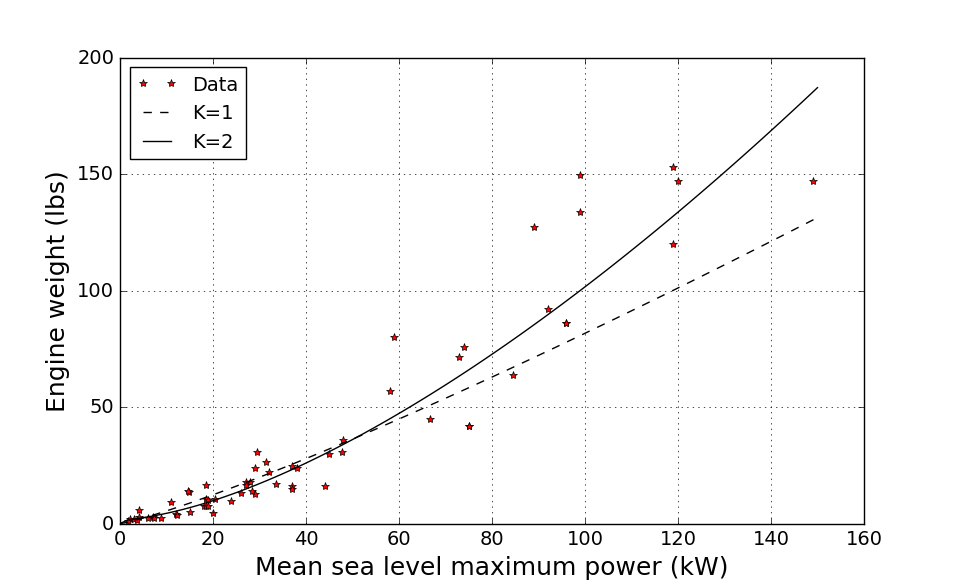
\includegraphics[width=0.8\textwidth]{enginePvsW.png}
    \caption{Engine MSL power versus weight fits for $K=1,2$ posynomial terms with underlying data.}
    \label{f:enginefit}
\end{figure}

With a SMA approximation, more terms do not improve the r.m.s.
error of the fit on the given data, due to the large standard deviation of the data used.
As such, we will proceed with the 2-term posynomial fit.

\subsubsection{Other constraints in engine model}

The cruise shaft power is constrained to be 20\% of the maximum shaft power of the engine,
to account for engine surge power demands and add engineering realism. This rather arbitrary constraint is removed
later when the full mission model is integrated.

\begin{equation}
    P_{shaft} \leq \frac{1}{5} P_{shaft,max}
\end{equation}

\subsection{Converting all subsystems into submodels}
\label{s:submodels}

Within this framework, we can modularize the SimPleAC into wing and fuselage modules as well,
with very little additional work. This creates the variable and constraint
hierarchy as presented in Figure~\ref{forest:submodels}, which define all of the constraints
required for SimPleAC to fly one flight segment.

\begin{figure}[!h]
    \centering\small\sffamily
    \begin{forest}
        sn edges
        [\textbf{Aircraft}
        [\textbf{Wing}]
        [\textbf{Fuselage}]
        [\textbf{Engine}]
        ]
    \end{forest}
    \caption{Variable and constraint hierarchy of the single mission segment SimPleAC model}
    \label{forest:submodels}
\end{figure}

Tree or graph structures such as in Figure~\ref{forest:submodels} are informative, since
it provides an intuitive representation of the way constraints and variables
are passed between GPkit models. In this basic framework,
variables and constraints from one model can only be called by models that are higher in
the tree diagram. This reconciles the fact that object creation in software engineering is serial, whereas
the components of the system being optimized are interconnected. The way the \gls{SP} is solved at the end has no
hierarchy, but as we will see in Section~\ref{s:mission} a hierarchical representation
will facilitate the vectorization of constraints required for mission design.

%TODO: develop on the idea of variable and constraint hierarchy

\section{Mission design and performance modeling form}
\label{s:mission}

The SimPleAC defined so far works well to demonstrate the
capabilities of \gls{SP} in helping explore tradeoffs in engineering design.
However, often in the design process, we will want to test the performance of a
design in different conditions, and/or during different phases of a mission.
This requires the vectorization of
constraints that relate to the performance of the design. What we'd like to do
is to have a single aircraft optimize both its static sizing variables (having
to do with the airframe), and its flight performance simultaneously. This requires a major
augmentation of the model tree defined in Figure~\ref{forest:submodels}, into a
uni-directional graph as shown in Figure~\ref{f:missiongraph}.

\begin{figure}[!h]
    \centering\small\sffamily
    \begin{forest}
        sn edges,
        l sep+=1em,
        s sep=(4-level)*4mm,
    [\textit{\textbf{Mission}},name=mission
    [\textit{\textbf{\shortstack{Aircraft\\Perf.}}},name=aircraftP1
    [\textit{\shortstack{Wing\\Perf.}},name=wingP1,tier=cp]
    [\textit{Atmosphere},name=atmos1,tier=a]
    [\textit{\shortstack{Engine\\Perf.}},name=engineP1,tier=cp]
    ]
    [\textbf{Aircraft},name=aircraft,tier=cp
    [\textbf{Wing},name=wing,tier=a]
    [\textbf{Fuselage},name=fuse,tier=a]
    [\textbf{Engine},name=engine,tier=a]
    ]
    [\textit{\textbf{\shortstack{Aircraft\\Perf.}}},name=aircraftP2
    [\textit{\shortstack{Wing\\Perf.}},name=wingP2,tier=cp]
    [\textit{Atmosphere},name=atmos2,tier=a]
    [\textit{\shortstack{Engine\\Perf.}},name=engineP2,tier=cp]
    ]
    ]
%
        \draw[->] (atmos1) -- (wingP1);
        \draw[->] (atmos1) -- (engineP1);
        \draw[->] (atmos2) -- (wingP2);
        \draw[->] (atmos2) -- (engineP2);
        \draw[->] (aircraft) -- (aircraftP1);
        \draw[->] (aircraft) -- (aircraftP2);
        \draw[->] (wing) -- (wingP1);
        \draw[->] (engine) -- (engineP1);
        \draw[->] (wing) -- (wingP2);
        \draw[->] (engine) -- (engineP2);
        \node[draw,rectangle,fit={(aircraftP2) (atmos2) (engineP2) (wingP2)},label=Segment 2] {};
        \node[draw,rectangle,fit={(aircraftP1) (atmos1) (engineP1) (wingP1)},label=Segment 1] {};
    \end{forest}
    \caption[Variable and constraint hierarchy of the SimPleAC model, for two flight
    segments.]{Variable and constraint hierarchy of the presented aircraft model, for two flight
    segments. Models that include sizing variables are
    bolded while models that include performance variables are italicized.
    There are models that contain both kinds of variables.}
    \label{f:missiongraph}
\end{figure}

Figure~\ref{f:missiongraph} represents a model with two flight segments, where the
models enclosed in rectangles contain the set of constraints that are vectorized
by the number of flight segments, $N_{segments} = 2$. Each
one of the performance models contain variables that change between flight segments.
Note that the fuselage is the only subcomponent not to have a performance model.
This is because the only performance variable of the fuselage is its drag
coefficient, which is assumed to not change between flight segments, making it static.
A \textbf{\textit{Mission}} model that links flight segments together has been added,
as well as an \textit{Atmosphere} model, which describes the conditions in which the aircraft
operates.

The static aircraft model and the atmospheric state are passed as an argument to multiple
performance models within this framework. To transform our previously static model to
the performance-static model hierarchy we have identified,
we have to determine which variables
belong in which node of the tree. Table~\ref{t:missionvars} details the full
decomposition of the model into its submodels in the format defined
by Figure~\ref{f:missiongraph}. This is as simple as identifying which variables
we do not expect to change during flight segments, and which ones we do. Note that
some of the variables from the previous sections
have been renamed (e.g.\ $T_{flight} \rightarrow t_m$ and $W_f \rightarrow W_{f_m}$)
to clarify their purpose within this framework.

\begin{center}
    \captionof{table}{Variables of SimPleAC in performance modeling, detailed in the
    variable and constraint hierarchy.}
    {\footnotesize
\begin{longtable}{lcl}
\toprule
Free Variables & Units & Description \\ \midrule
\multicolumn{3}{l}{\textbf{Mission}} \\
$W_{f_{m}}$ & $~\mathrm{N}$ & Total mission fuel \\
$t_m$ & $~\mathrm{hr}$ & Total mission time \\
$R_s$ & $~\mathrm{km}$ & Range flown in segment \\
$W_{avg}$ & $~\mathrm{N}$ & Segment average weight \\
$W_{end}$ & $~\mathrm{N}$ & Weight at the end of flight segment \\
$W_{f_s}$ & $~\mathrm{N}$ & Segment fuel burn \\
$W_{start}$ & $~\mathrm{N}$ & Weight at the beginning of flight segment \\
$\frac{\Delta h}{dt}$ & $~\mathrm{\tfrac{m}{hr}}$ & Climb rate \\
$h$ & $~\mathrm{m}$ & Flight altitude \\
$t_s$ & $~\mathrm{hr}$ & Time spent in flight segment \\
\hline
\multicolumn{3}{l}{\textbf{Mission/Atmosphere}} \\
$\mu$ & $~\mathrm{\tfrac{kg}{\left(m\cdot s\right)}}$ & dynamic viscosity \\
$\rho$ & $~\mathrm{\tfrac{kg}{m^{3}}}$ & density of air \\
$h$ & $~\mathrm{m}$ & altitude \\
\hline
\multicolumn{3}{l}{\textbf{Mission/SimPleAC}} \\
$V_f$ & $~\mathrm{m^{3}}$ & maximum fuel volume \\
$V_{f_{avail}}$ & $~\mathrm{m^{3}}$ & fuel volume available \\
$W$ & $~\mathrm{N}$ & maximum takeoff weight \\
$W_f$ & $~\mathrm{N}$ & maximum fuel weight \\
\hline
\multicolumn{3}{l}{\textbf{Mission/SimPleAC/Engine}} \\
$P_{shaft_{max}}$ & $~\mathrm{kW}$ & MSL maximum shaft power \\
$W_e$ & $~\mathrm{N}$ & engine weight \\
\hline
\multicolumn{3}{l}{\textbf{Mission/SimPleAC/Fuselage}} \\
$(CDA0)$ & $~\mathrm{m^{2}}$ & fuselage drag area \\
$C_{D_{fuse}}$ & $$ & fuselage drag coefficient \\
$V_{f_{fuse}}$ & $~\mathrm{m^{3}}$ & fuel volume in the fuselage \\
\hline
\multicolumn{3}{l}{\textbf{Mission/SimPleAC/Wing}} \\
$A$ & $$ & aspect ratio \\
$S$ & $~\mathrm{m^{2}}$ & total wing area \\
$V_{f_{wing}}$ & $~\mathrm{m^{3}}$ & fuel volume in the wing \\
$W_w$ & $~\mathrm{N}$ & wing weight \\
$W_{w_{strc}}$ & $~\mathrm{N}$ & wing structural weight \\
$W_{w_{surf}}$ & $~\mathrm{N}$ & wing skin weight \\
\hline
\multicolumn{3}{l}{\textbf{Mission/SimPleACP}} \\
$C_D$ & $$ & drag coefficient \\
$D$ & $~\mathrm{N}$ & total drag force \\
$L/D$ & $$ & lift-to-drag ratio \\
$Re$ & $$ & Reynolds number \\
$V$ & $~\mathrm{\tfrac{m}{s}}$ & cruising speed \\
\hline
\multicolumn{3}{l}{\textbf{Mission/SimPleACP/EngineP}} \\
$P_{shaft}$ & $~\mathrm{kW}$ & shaft power \\
$T$ & $~\mathrm{N}$ & propeller thrust \\
\hline
\multicolumn{3}{l}{\textbf{Mission/SimPleACP/WingP}} \\
$C_L$ & $$ & wing lift coefficient \\
$C_f$ & $$ & skin friction coefficient \\
$C_{D_{ind}}$ & $$ & wing induced drag \\
$C_{D_{wpar}}$ & $$ & wing profile drag \\
\bottomrule
\end{longtable}}

{\footnotesize
\begin{longtable}{lcl}
\toprule
Constants & Units & Description \\ \midrule
\multicolumn{3}{l}{\textbf{Mission}} \\
$Cost Index$ & $~\mathrm{\tfrac{1}{hr}}$ & hourly cost index \\
$Range$ & $~\mathrm{km}$ & aircraft range \\
$V_{min}$ & $~\mathrm{\tfrac{m}{s}}$ & takeoff speed \\
$W_p$ & $~\mathrm{N}$ & payload weight \\
\hline
\multicolumn{3}{l}{\textbf{Mission/Atmosphere}} \\
$P_{MSL}$ & $~\mathrm{Pa}$ & pressure at MSL \\
$T_{MSL}$ & $~\mathrm{K}$ & temperature at MSL \\
$\mu_{MSL}$ & $~\mathrm{\tfrac{kg}{\left(m\cdot s\right)}}$ & dynamic viscosity at MSL \\
$\nu_{MSL}$ & $~\mathrm{\tfrac{m^{2}}{s}}$ & kinematic viscosity at MSL \\
$\rho_{MSL}$ & $~\mathrm{\tfrac{kg}{m^{3}}}$ & density of air at MSL \\
$a_{MSL}$ & $~\mathrm{\tfrac{m}{s}}$ & Speed of sound at MSL \\
$h_{top}$ & $~\mathrm{m}$ & highest altitude valid \\
\hline
\multicolumn{3}{l}{\textbf{Mission/SimPleAC}} \\
$\rho_f$ & $~\mathrm{\tfrac{kg}{m^{3}}}$ & density of fuel \\
$g$ & $~\mathrm{\tfrac{m}{s^{2}}}$ & gravitational acceleration \\
\hline
\multicolumn{3}{l}{\textbf{Mission/SimPleAC/Engine}} \\
$P_{shaft_{ref}}$ & $~\mathrm{kW}$ & reference MSL maximum shaft power \\
$W_{e_{ref}}$ & $~\mathrm{N}$ & reference engine weight \\
$\eta_{prop}$ & $$ & propeller efficiency \\
\hline
\multicolumn{3}{l}{\textbf{Mission/SimPleAC/Wing}} \\
$(\frac{S}{S_{wet}})$ & $$ & wetted area ratio \\
$C_{L,max}$ & $$ & max CL with flaps down \\
$N_{ult}$ & $$ & ultimate load factor \\
$W_{w_{coeff1}}$ & $~\mathrm{\tfrac{1}{m}}$ & wing weight coefficent 1 \\
$W_{w_{coeff2}}$ & $~\mathrm{Pa}$ & wing weight coefficent 2 \\
$\tau$ & $$ & airfoil thickness to chord ratio \\
$e$ & $$ & Oswald efficiency factor \\
$k$ & $$ & form factor \\
\hline
\multicolumn{3}{l}{\textbf{Mission/SimPleACP/EngineP}} \\
$BSFC$ & $~\mathrm{\tfrac{g}{\left(hr\cdot kW\right)}}$ & thrust specific fuel consumption \\
\bottomrule
\end{longtable}}
{\footnotesize
\begin{longtable}{lcl}
\toprule
Sensitivities & Units & Description \\ \midrule
\multicolumn{3}{l}{\textbf{Mission}} \\
$Range$ & $~\mathrm{km}$ & aircraft range \\
$V_{min}$ & $~\mathrm{\tfrac{m}{s}}$ & takeoff speed \\
$Cost Index$ & $~\mathrm{\tfrac{1}{hr}}$ & hourly cost index \\
$W_p$ & $~\mathrm{N}$ & payload weight \\
\hline
\multicolumn{3}{l}{\textbf{Mission/Atmosphere}} \\
$\rho_{MSL}$ & $~\mathrm{\tfrac{kg}{m^{3}}}$ & density of air at MSL \\
$\mu_{MSL}$ & $~\mathrm{\tfrac{kg}{\left(m\cdot s\right)}}$ & dynamic viscosity at MSL \\
$h_{top}$ & $~\mathrm{m}$ & highest altitude valid \\
\hline
\multicolumn{3}{l}{\textbf{Mission/SimPleAC}} \\
$g$ & $~\mathrm{\tfrac{m}{s^{2}}}$ & gravitational acceleration \\
$\rho_f$ & $~\mathrm{\tfrac{kg}{m^{3}}}$ & density of fuel \\
\hline
\multicolumn{3}{l}{\textbf{Mission/SimPleAC/Engine}} \\
$\eta_{prop}$ & $$ & propeller efficiency \\
$P_{shaft_{ref}}$ & $~\mathrm{kW}$ & reference MSL maximum shaft power \\
$W_{e_{ref}}$ & $~\mathrm{N}$ & reference engine weight \\
\hline
\multicolumn{3}{l}{\textbf{Mission/SimPleAC/Wing}} \\
$(\frac{S}{S_{wet}})$ & $$ & wetted area ratio \\
$k$ & $$ & form factor \\
$C_{L,max}$ & $$ & max CL with flaps down \\
$e$ & $$ & Oswald efficiency factor \\
$\tau$ & $$ & airfoil thickness to chord ratio \\
$W_{w_{coeff2}}$ & $~\mathrm{Pa}$ & wing weight coefficent 2 \\
$N_{ult}$ & $$ & ultimate load factor \\
$W_{w_{coeff1}}$ & $~\mathrm{\tfrac{1}{m}}$ & wing weight coefficent 1 \\
\hline
\multicolumn{3}{l}{\textbf{Mission/SimPleACP/EngineP}} \\
$BSFC$ & $~\mathrm{\tfrac{g}{\left(hr\cdot kW\right)}}$ & thrust specific fuel consumption \\
\bottomrule
\end{longtable}}

    \label{t:missionvars}
\end{center}

Then, using the variable structure in Table~\ref{t:missionvars}, we can place the
constraints in the appropriate locations. Each constraint should be placed
in the model that contains the variable in the constraint that is highest in the level of hierarchy. For example,
we can consider the constraint for thrust power in Equation~\ref{e:thrustConstr}.

\begin{equation}
    \label{e:thrustConstr}
    T \times V \leq \eta_{prop} P_{shaft}
\end{equation}

We expect that thrust ($T$) and shaft power ($P_{shaft}$) occur
in \textit{Engine Performance}. Since our model has no model for propeller efficiency ($\eta_{prop}$), we treat it
as a static variable in \textbf{Engine}. And velocity ($V$) is a variable in \textbf{\textit{Aircraft {Performance}}}.
As a result, the constraint for thrust power would logically reside in the \textbf{\textit{Aircraft {Performance}}}
model, the highest level in the hierarchy as shown in Figure~\ref{f:thrustConstr}. Since this model is vectorized,
the constraint would be vectorized by the number of flight segments we create.

\begin{figure}[!h]
    \centering\small\sffamily
    \begin{forest}
        sn edges,
        l sep+=1em,
        s sep=(4-level)*4mm,
        for children={
        l sep+=1em,
        }
    [\textit{\textbf{Mission}},name=mission
    [\textit{\textbf{\shortstack{Aircraft\\Perf.}}},name=aircraftP
    [\textit{\shortstack{Wing\\Perf.}},name=wingP,tier=cp]
    [\textit{Atmosphere},name=atmos,tier=a]
    [\textit{\shortstack{Engine\\Perf.}},name=engineP,tier=cp]
    ]
    [\textbf{Aircraft},name=aircraft,tier=cp
    [\textbf{Wing},name=wing,tier=a]
    [\textbf{Fuselage},name=fuse,tier=a]
    [\textbf{Engine},name=engine,tier=a]
    ]
    ]
        \draw[->] (atmos) -- (wingP);
        \draw[->] (atmos) -- (aircraftP);
        \draw[->] (aircraft) -- (aircraftP);
        \draw[->] (aircraft) -- (mission);
        \draw[->] (wing) -- (wingP);
        \draw[->] (engine) -- (engineP);
        \node[draw,circle,fit={(engineP)}, inner sep=-1pt] {};
        \node[draw,circle,fit={(aircraftP)}, inner sep=-1pt] {};
        \node[draw,circle,fit={(engine)}, inner sep=-1pt] {};
        \node[draw,rectangle,fit={(aircraftP) (engineP) (wingP) (atmos)},label=below:{Segment}] {};
    \end{forest}
    \caption[Variable hierarchy of thrust constraint~\ref{e:thrustConstr}.]{Variable hierarchy
    of thrust constraint~\ref{e:thrustConstr}. The models
    that contain the variables in the constraint are enclosed in circles.
    Constraint logically resides in \textbf{\textit{Aircraft Perf.}}.
    The vectorization of flight segment performance models in the
    rectangle has been neglected for clarity.}
    \label{f:thrustConstr}
\end{figure}

Now we have used a framework to modularize our constraints, which makes it
amenable to vectorization and mission design.

\subsection{Linking performance models: flight segments}

Although the variables in the performance models are vectorized, they can be constrained
against each other. If each of the \textit{\textbf{Aircraft Performance}} models were operating
independently of
each other simulating different missions, then they would simply be merged in the bag of constraints
of \textbf{\textit{Mission}}. However, we know that the models are related since the aircraft
burns fuel throughout the mission, changing its flight characteristics.

The derivation of the \gls{SP}-compatible flight segment models has been detailed in~\cite{sp_ac_design},
and used widely within the \gls{CEG} in aircraft design.
%However, the model in ~\cite{sp_ac_design} makes the distinction between cruise and climb flight segments
%which we do not desire for this design problem since we would like to be able to optimize the entire
%flight profile.
It defines segment start, end and average weights,
as well as altitude, and all of its relevant constraints are contained in the \textbf{\textit{Mission}}
model. Please find the full set of variables belonging to the flight segment model in Appendix~\ref{a:flightprofilevars}.

The monomial equality below has been added to the formulation

\begin{align}
    h_{{avg}_1} &= \frac{1}{2}\Delta h_1 \\
    h_{{avg}_i} &= \sqrt{h_{i} \times h_{i-1}}, \quad i = 2,...,N_{segments}
\end{align}

to define an average altitude variable $h_{avg}$ with respect to the segment altitude change variable $\Delta h$
and segment ending altitude $h$
in Section~\ref{s:atmos}. This adds
conservatism to the density and drag (otherwise, the air density for a flight segment is calculated
at the end of the segment, at which the aircraft is at its highest altitude).
The cruise altitude (final altitude in every flight segment but the initial segment) has been constrained
to be greater than 5000m.

As with most \gls{GP} approximations, there are limitations to this model. To avoid non-positive
altitude change values ($\Delta h$), we restrict the aircraft to climb during every segment, and
don't model descents. Furthermore, we have binned the flight segments to equal range segments to
avoid the potential lower-unboundedness of the lengths of certain segments.

\subsection{Characterizing the environment: atmospheric model}
\label{s:atmos}

We have created a mission and flight segment framework without having a model
of the environment in which the aircraft operates. So far, we have assumed that
the aircraft flies at a constant altitude (sea level) for a single mission segment,
and is subject to the same air density and viscosity.
An atmospheric model is essential to capturing the tradeoffs between flight altitude, engine performance,
and lift and drag characteristics.
This simplification is overcome through vectorization.

Tony Tao's atmosphere fits have been borrowed for this purpose~\cite{tao_thesis}. These are
2-term softmax-affine fits of the atmospheric
quantities of interest ($\rho$ and $\mu$ in this thesis) with respect to altitude. The constraints
are guaranteed to be tight through signomial equalities, as explained in Section~\ref{s:sigeq}.
The relations are valid between 0-10000m of altitude.

Similar environmental models can be made for other design problems where the environmental
variables are inextricably coupled to performance. Another good example of environmental modeling
in \gls{GP} is performed by Burton~\cite{gassolar}, where wind speeds are integrated into
a loitering aircraft optimization problem.

\subsection{Objective of the mission model}
\label{s:missionobj}

Recalling from Section~\ref{s:altobj}, upper-unbounded performance metrics often have to
reside in the objective function to be bounded. We combine mission fuel $W_{f_m}$ and mission time $t_m$
into a composite objective function through a cost index $C$ for boundedness,

\begin{equation}
    \mathrm{Objective} \geq W_f \frac{1}{\mathrm{N}} + \mathrm{C} \times t_m
    \label{e:missionobj}
\end{equation}

and divide $W_{f_m}$ by newtons to achieve uniform units (non-dimensional).
Another method to achieve proper boundedness is to add an arbitrary large upper bound. However
this will result in the bounding constraint being tight and giving unphysical results, and so
this thesis will implement the objective in~\ref{e:missionobj} instead.
Cost index $\mathrm{C}$ is defined as a separate parameter so that we can observe the sensitivity
of the variable post-optimization.

\section{Design exploration through mission design}

There are a few interesting methods that we can use to explore
potential designs using~\gls{GP}s. So instead of showing the single optimum of the
SimPleAC with a full mission profile, leveraging the speed of convex optimization,
we can map out the entire design space with respect to variables of interest.
Please refer to~\cite{power_of_log} for details on the computational advantages of the \gls{GP}
and \gls{SP} compared to other non-linear optimization methods.

In this case, the SimPleAC has been optimized
over a range of payload weight (1000-10000 N) and range (1000-5000km), and the mission fuel weight
and total weight have been plotted in contour plots in Figure~\ref{f:pareto}. Note that
every point in the design space represents a fully optimized aircraft. The full list of inputs
to the \textbf{\textit{Mission}} model are detailed in Table~\ref{t:sweepinputs}

\begin{footnotesize}
        \begin{table}
            \centering
            \begin{tabular}{llcl}
                \toprule
                Constants & Value & Units & Description\\ \midrule
                $Range$ & [1000-10000]  & $~\mathrm{km}$ & aircraft range \\
                $W_p$ & [1000-5000]  & $~\mathrm{N}$ & payload weight \\
                $C$ & 120 & $~\mathrm{\tfrac{1}{hr}}$ & hourly cost index \\
                $T/O factor$ & 2 & $$ & takeoff thrust factor \\
                $V_{min}$ & 25 & $~\mathrm{\tfrac{m}{s}}$ & takeoff speed \\
                $h_{cruise}$ & 5000 & $~\mathrm{m}$ & minimum cruise altitude \\
            \end{tabular}
            \caption{Inputs to the design space exploration of the \textbf{\textit{Mission}} model.}
            \label{t:sweepinputs}
        \end{table}
\end{footnotesize}

\begin{figure*}[t!]
    \centering
    \begin{subfigure}[t]{0.5\linewidth}
        \centering
        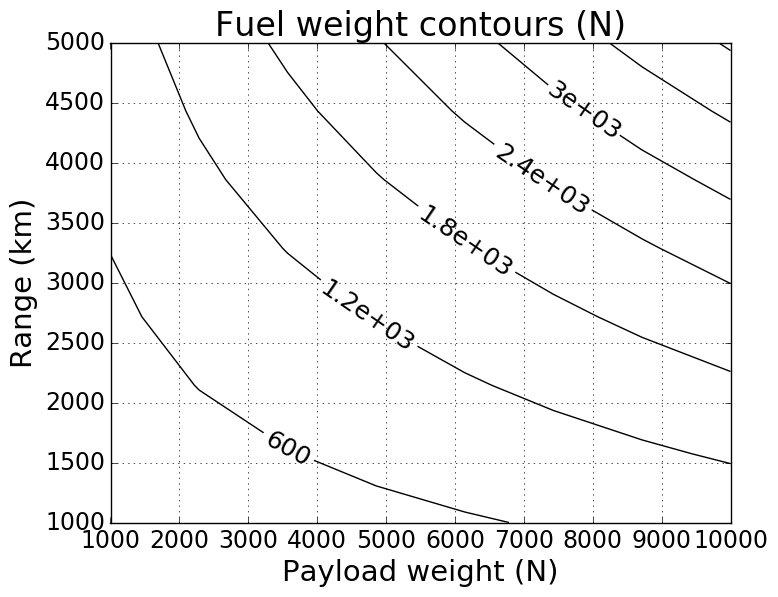
\includegraphics[width=0.95\linewidth]{mission2/Wfcontours.png}
    \end{subfigure}%
    ~
    \begin{subfigure}[t]{0.5\linewidth}
        \centering
        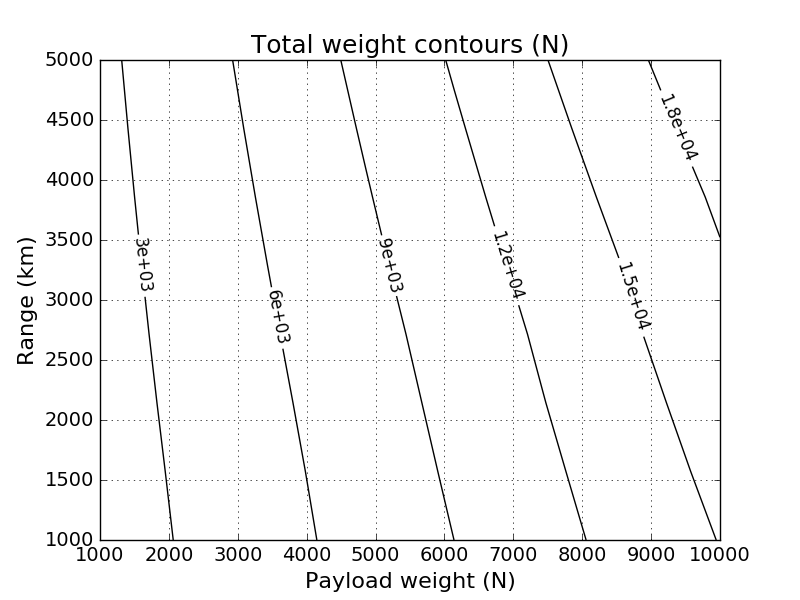
\includegraphics[width=0.95\linewidth]{mission2/Wcontours.png}
    \end{subfigure}
    \caption{The fuel and total weight contours with respect to range and payload.}
    \label{f:pareto}
\end{figure*}

In Section~\ref{s:fuel} we had to weigh whether or not it was worth losing the mathematical
guarantees of convexity to be able to model fuel storage. Now we can use our \gls{SP} model to understand
the tradeoffs in fuel storage, and when it is beneficial to store fuel in the wing versus the fuselage.

\begin{figure}
    \centering
    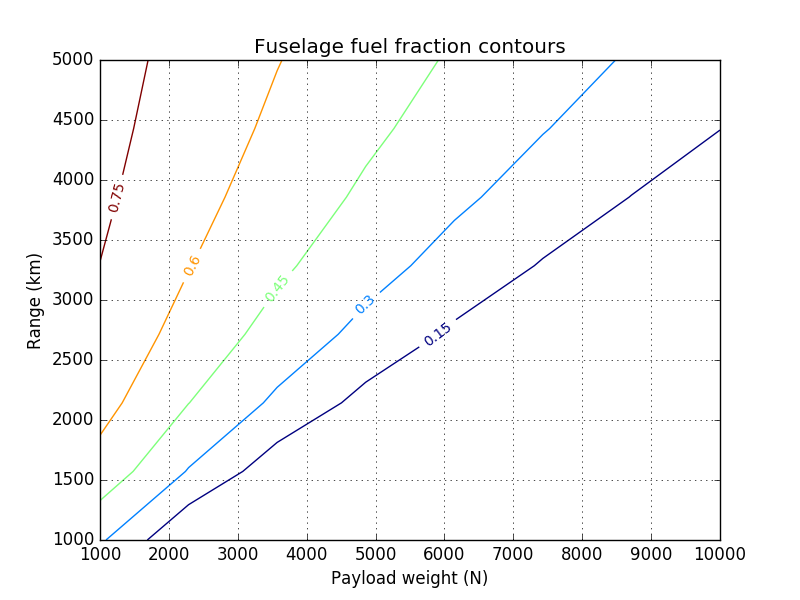
\includegraphics[width=0.475\linewidth]{mission2/vffusefraccontours.png}
    \caption{Fraction of total fuel stored in fuselage with respect to range and payload.}
    \label{f:fusefuelfrac}
\end{figure}

Figure~\ref{f:fusefuelfrac} shows how designs for different range and payload requirements
allocate fuel differently within the aircraft. As the mission range increases for a given payload weight
(upward movement on the graph),
more and more fuel is allocated within the fuselage as a proportion of total fuel. Since fuselage fuel
volume is directly related to increased fuselage drag, it is logical that no fuel is put in the fuselage
until the fuel volume constraint in the wing becomes tight. And this is the behavior that is observed,
since no fuel is allocated in the fuselage towards the lower right of the graph.

\begin{figure*}[t!]
    \centering
    \begin{subfigure}[t]{0.5\linewidth}
        \centering
        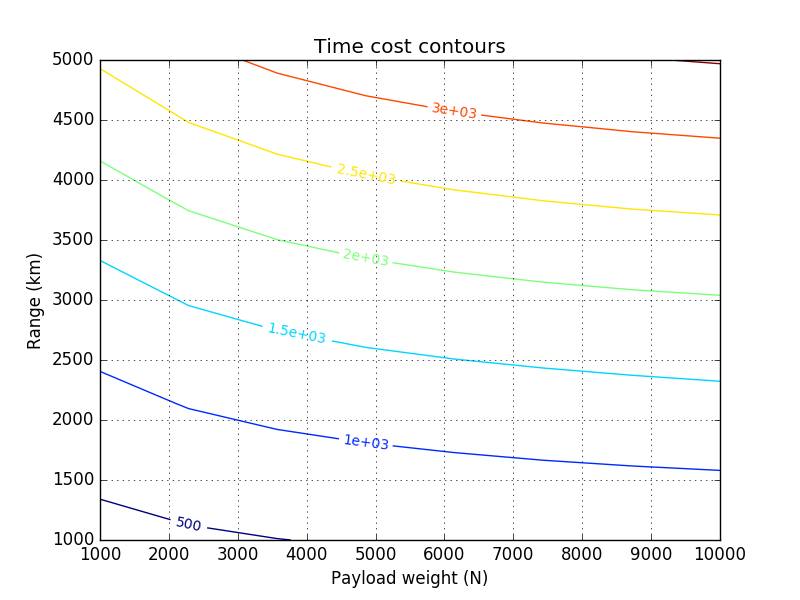
\includegraphics[width=0.95\linewidth]{mission2/timecostcontours.png}
    \end{subfigure}%
    ~
    \begin{subfigure}[t]{0.5\linewidth}
        \centering
        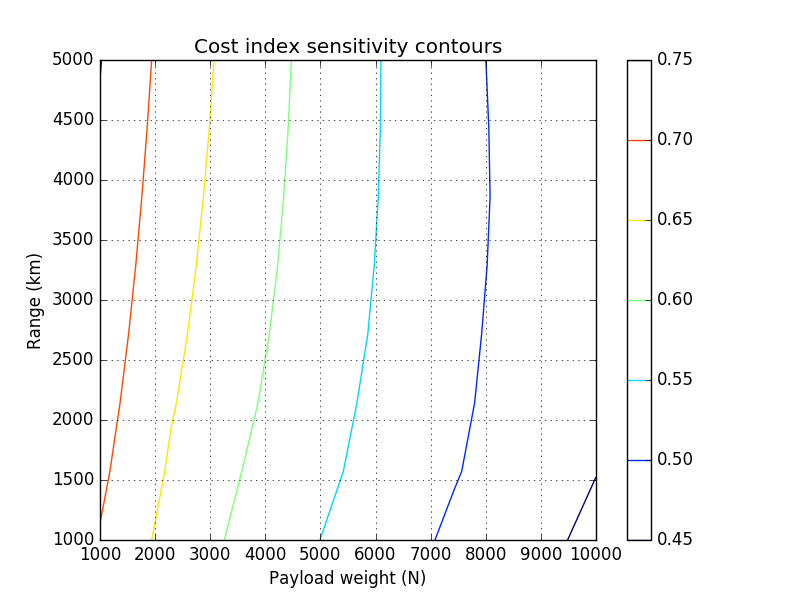
\includegraphics[width=0.95\linewidth]{mission2/Csenscontours.png}
    \end{subfigure}
    \caption[Time cost and time cost index sensitivity contours.]{Time cost and time cost index sensitivity contours.
    We can gain intuition about the relative importance of different components
    of composite objective functions by showing both the costs and their sensitivities together.}
    \label{f:compobjsens}
\end{figure*}

For composite objective functions, it can be difficult to have intuitions about how sensitivities
to parameters can affect the design, since the parameters act on multiple variables of interest. A way
to attempt to decouple these is to plot both the cost of a variable in the objective and its relevant
sensitivity next to each other, as shown in Figure~\ref{f:compobjsens}. Taking a look at point [4000N,4000km],
we can follow the yellow contour to see all of the missions with the same time cost as this mission
(same average flight speed),
and see how the fraction of time cost versus total cost varies through the sensitivity to the time cost index.
This can help a designer gain intuition about the relative importance of different components of cost.

\section{More modeling improvements before multimission design}

There are still significant weaknesses in the model relating to the engine of the model that require
improvement before we can perform multimission design in Section~\ref{s:multimission}.
We can see this by observing the sensitivities in Table~\ref{t:sens}.

    \begin{table}
        \footnotesize
        \centering
        \begin{tabular}{l c l}
            \toprule
            Variable/Model & Sensitivity & Variable description \\ \midrule
            \multicolumn{3}{l}{\textbf{Mission}} \\
            $Range$ & +1.1 & aircraft range \\
            $V_{min}$ & -0.67 & takeoff speed \\
            $C$ & +0.46 & hourly cost index \\
            $W_p$ & +0.45 & payload weight \\
            $h_{cruise}$ & +0.12 & minimum cruise altitude \\
            & & \\
            \multicolumn{3}{l}{\textbf{Mission/SimPleAC}} \\
            $g$ & +0.54 & gravitational acceleration \\
            $\rho_f$ & -0.042 & density of fuel \\
            & & \\
            \multicolumn{3}{l}{\textbf{Mission/SimPleAC/Engine}} \\
            $\eta_{prop}$ & -0.65 & propeller efficiency \\
            $P_{shaft,ref}$ & -0.067 & reference MSL maximum shaft power \\
            $W_{e,ref}$ & +0.044 & reference engine weight \\
            & & \\
            \multicolumn{3}{l}{\textbf{Mission/SimPleAC/Wing}} \\
            $(\frac{S}{S_{wet}})$ & +0.45 & wetted area ratio \\
            $k$ & +0.45 & form factor \\
            $C_{L,max}$ & -0.33 & lift coefficient at stall \\
            $e$ & -0.17 & Oswald efficiency factor \\
            $W_{w_{coeff2}}$ & +0.12 & wing weight coefficient 2 \\
            $\tau$ & -0.11 & airfoil thickness to chord ratio \\
            $N_{ult}$ & +0.07 & ultimate load factor \\
            $W_{w_{coeff1}}$ & +0.07 & wing weight coefficient 1 \\
            & & \\
            \multicolumn{3}{l}{\textbf{Mission/SimPleACP/EngineP}} \\
            $BSFC$ & [ +0.16 +0.14 +0.14 +0.14    ] & brake specific fuel consumption \\
            \bottomrule
        \end{tabular}
        \caption{A selection of sensitivities of the solution to design parameters.}
        \label{t:sens}
    \end{table}

As we can see, variables internal to the engine model, such as \BSFC and $\eta_{prop}$ have
large sensitivities (0.59 and -0.65 respectively). The objective of the model
is as sensitive to these variables as mission input variables such as range and payload, so
these variables require refinement.

The following sections will take a two-pronged approach to improved engine modeling.
The first weakness of the current model is the fact that the engine can supply the same amount of power
regardless of altitude. The maximum power of naturally aspirated piston engines drops
with altitude; adding a lapse rate will improve how much we trust the engine model.
The second weakness is the lack of an engine \BSFC model. Empirical data shows that the
\BSFC of an engine deteriorates at low power outputs.
In Sections~\ref{s:lapse} and \ref{s:BSFC}, these improvements will be implemented using more data-based modeling.

\subsection{Engine lapse rate model}
\label{s:lapse}

Data-based modeling techniques have been detailed in Section~\ref{s:datafit}.
In the same way posynomial fits were created for the relationship between
engine maximum power and weight, the lapse rate of the engine was fitted with respect to throttle level.
This model requires the insertion of another signomial equality into the model. Consider the
posynomial inequality expression below:

\begin{equation}
    \label{e:lapse}
    1 \geq L + \frac{P_{shaft,alt}}{P_{shaft,max}}
\end{equation}

Since the \BSFC of a normally aspirated piston engine would be expected to improve
as the $P_{shaft} \xrightarrow[]{} P_{shaft,alt}$, the maximum shaft
power at altitude has downward pressure on it from the fuel burn objective. This means that the
inequality doesn't adequately lower-bound the $P_{shaft,alt}$. If we try to flip the inequality in
Constraint~\ref{e:lapse}, then $P_{shaft,alt}$ is upper-unbounded, so with our current parametrization
of the shaft power, we must use a signomial equality.

\subsection{Making use of sensitivities: engine \BSFC model}
\label{s:BSFC}

The \BSFC is one of the variables that the model is most sensitive to (total sensitivity over all mission segments of 0.59),
and it has yet to be modeled. As
stated in Section~\ref{s:lapse}, the \BSFC of a naturally-aspirated piston engine improves as the engine
puts out more power relative to its maximum power at a given altitude.

BSFC has downward pressure due to the objective function, and therefore must be lower-bounded. This makes
it amenable to multiple-term posynomial fits.

First, a monomial fit of the $\frac{\BSFC}{\BSFC_{min}}$ versus $\frac{P_{shaft}}{P_{shaft,alt}}$ was created.
The result is shown by the green line in Figure~\ref{f:P_BSFC}.

\begin{figure}
    \centering
    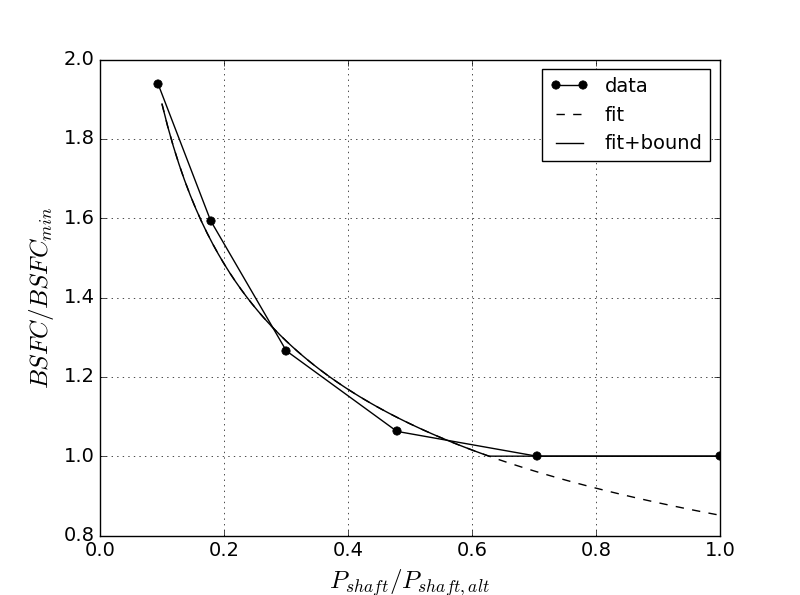
\includegraphics[width=0.6\textwidth]{P_BSFC.png}
    \caption[$\frac{\BSFC}{\BSFC_{min}}$ versus $\frac{P_{shaft}}{P_{shaft,alt}}$ data fit.]{$\frac{\BSFC}{\BSFC_{min}}$ versus $\frac{P_{shaft}}{P_{shaft,alt}}$ data fit. The green fit is
    not able to capture the tail ends of the curve, which is resolved by the bounding in the red fit.}
    \label{f:P_BSFC}
\end{figure}

Although the r.m.s. error of the fit is low (0.028) due to the small number of data points (in blue),
there is a significant deterioration in the quality of the
fit as $\frac{P_{shaft}}{P_{shaft,alt}} \xrightarrow[]{} 1$,
and increasing the number of posynomial terms in the fit does not alleviate this problem.
What we can do is put a lower bound on the \BSFC of the engine that depends on the actual
lowest \BSFC achieved by the engine. The final \BSFC relation is shown in Equation~\ref{e:BSFCfit}.

\begin{equation}
    \label{e:BSFCfit}
    \left(\frac{\BSFC}{\BSFC_{min}}\right)^{0.1} = .984\left(\frac{P_{shaft}}{P_{shaft,alt}}\right)^{-0.0346},~
    \left(\frac{\BSFC}{\BSFC_{min}}\right) \geq 1
\end{equation}

\section{Multimission design}
\label{s:multimission}

Having created a mission profile for the SimPleAC, it only takes one extra level of
hierarchy to do multimission design. Now we vectorize the mission models flown by the same aircraft.

\begin{figure}[!h]
    \centering\small\sffamily
    \begin{forest}
        sn edges,
        l sep+=1em,
        s sep=(4-level)*5mm,
        for children={
        l sep+=1em,
        }
        [\textit{\textbf{Multimission}},name=multimission
        [\textit{\textbf{Mission}},name=mission1
        [\textit{\textbf{\shortstack{Aircraft\\Perf.}}},tikz={\node [draw,fit=()(!1),label=below:{Segment 1}] {};},name=ap1
        [,name=ap1d,edge=dotted,tier=p]]
        [\textit{\textbf{\shortstack{Aircraft\\Perf.}}},tikz={\node [draw,fit=()(!1),label=below:{Segment 2}] {};},name=ap2
        [,name=ap2d,edge=dotted,tier=p]]
        ]
        [\textbf{Aircraft},name=ac,tier=p
        [,name=ad,edge=dotted]]
        [\textit{\textbf{Mission}},name=mission2
        [\textit{\textbf{\shortstack{Aircraft\\Perf.}}},tikz={\node [draw,fit=()(!1),label=below:{Segment 1}] {};},name=ap3
        [,name=ap3d,edge=dotted,tier=p]]
        [\textit{\textbf{\shortstack{Aircraft\\Perf.}}},tikz={\node [draw,fit=()(!1),label=below:{Segment 2}] {};},name=ap4
        [,name=ap4d,edge=dotted,tier=p]]
        ]
        ]
        \draw[->] (ac) -- (ap1);
        \draw[->] (ac) -- (ap2);
        \draw[->] (ac) -- (ap3);
        \draw[->] (ac) -- (ap4);
        \draw[->] (ac) -- (mission1);
        \draw[->] (ac) -- (mission2);
        \node[draw,circle,fit={(mission1) (ap1) (ap2) (ap1d) (ap2d)},inner sep=0.34cm,label=Mission 1] {};
        \node[draw,circle,fit={(mission2) (ap3) (ap4) (ap3d) (ap4d)},inner sep=0.34cm,label=Mission 2] {};
    \end{forest}
    \caption{Multimission uni-directional graph, with $N_{segments} = 2$ and $N_{missions} = 2$.}
    \label{f:multimission}
\end{figure}

Now the vectorization has gone down two levels, where each performance model is vectorized $N_{segments} \times N_{missions}$ times,
and each mission model is vectorized $N_{missions}$ times. The single instance of \textbf{Aircraft}
is passed on as an argument to all of these models, which ensures that both its
static and performance constraints are satisfied for each flight segment
of every mission.

\subsection{Multimission objective functions}

The objective function of the \textbf{\textit{Multimission}} model has to be
a posynomial that puts pressure on the variables in every \textbf{\textit{Mission}} model. For example, knowing that
$W_{f_m} \frac{1}{\mathrm{N}} + C \times t_{m}$ is a valid objective functions to the single mission,
the objective function below for $N_{missions}$

\begin{equation}
    \mathrm{Objective} \geq \sum_{n=1}^{N_{missions}} W_{f_m} \frac{1}{\mathrm{N}} + \mathrm{C} \times t_{m}
    \label{e:compObj}
\end{equation}

will definitely work, since the same aircraft will fulfill two missions that are thus linked.
Assuming that $N_{missions} = 2$, note that an objective of the type below will also work

\begin{equation}
    \mathrm{Objective} \geq W_{f_{m_{1}}} \frac{1}{\mathrm{N}} + \mathrm{C}_{2} \times t_{m_{2}}
    \label{e:sepObj}
\end{equation}

but will require some management in variable boundedness since some internal variables,
namely  $W_{f_{m_{2}}}$ and $t_{m_{1}}$, can and will diverge to numerical infinity since they
are not necessarily pressured by the objective function.
Simply upper-bounding the variables
internally by some large bound will resolve boundedness issues. For this kind of objective, the
performance of the aircraft will be a compromise with respect to aircraft optimized purely
for mission time for the first mission or fuel burn for the second mission.

\subsection{Multimission optimization results}

The SimPleAC was optimized for the 3 different mission scenarios:

\begin{enumerate}
    \item M1: A single mission minimizing fuel burn ($W_{f_m}$).
    \item M2: A single mission minimizing time cost ($\mathrm{C} \times t_{m}$)
    \item MM: A multimission design performing both missions, minimizing fuel burn over M1 ($W_{f_{m_1}}$), and mission
                    time over M2 ($\mathrm{C}_{2} \times t_{m_{2}}$) (objective in Equation~\ref{e:sepObj}).
\end{enumerate}

The different mission requirements are detailed in Table~\ref{t:mminputs}. M1 is the same mission as
the one specified in Section~\ref{s:mission}, simulating a standard ferry mission where we care about fuel
consumption. M2 is a dash mission delivering more payload than M1, where mission time is the objective. Both missions
share the same flight altitudes, takeoff thrust factors and minimum takeoff speeds.

\begin{footnotesize}
\begin{center}
\begin{longtable}{lllcl}
\toprule
Input & M1 & M2 & Units & Description\\ \midrule
$C$ & 120 & 360  & $~\mathrm{\tfrac{1}{hr}}$ & hourly cost index \\
$Range$ & 3000 & 1000  & $~\mathrm{km}$ & aircraft range \\
$W_p$ & 6250 & 8000  & $~\mathrm{N}$ & payload weight \\
$h_{cruise}$ & \multicolumn{2}{c}{5000} & $~\mathrm{m}$ & minimum cruise altitude \\
$T/O factor$ & \multicolumn{2}{c}{2} & $$ & takeoff thrust factor \\
$V_{min}$ & \multicolumn{2}{c}{25} & $~\mathrm{\tfrac{m}{s}}$ & takeoff speed \\
    \caption{Inputs to the M1 and M2 \textbf{\textit{Mission}} models.}
    \label{t:mminputs}
\end{longtable}
\end{center}
\end{footnotesize}

The results are shown in Table~\ref{t:mmoutputs}.
The multimission aircraft represents a compromise aircraft that performs both missions
with relatively high performance.

\begin{center}
    \captionof{table}{Results of the single- and multi- mission solutions. Italicized values
    have been post-processed.}
    \begin{footnotesize}
\begin{longtable}{lllllcl}
\toprule
Variables & M1 & M2 & MM1 & MM2 & Units & Description \\
\midrule
$W$ & 10453 & 45199 & \multicolumn{2}{c}{13843} & $~\mathrm{N}$ & maximum takeoff weight \\
$AR$ & 18.6 & 1.66 & \multicolumn{2}{c}{7.53} & $~\mathrm{-}$ & aspect ratio \\
$S$ & 27.8 & 120.2 & \multicolumn{2}{c}{36.8} & $~\mathrm{m^{2}}$ & total wing area \\
$W_e$ & 72 & 22730 & \multicolumn{2}{c}{1425} & $~\mathrm{N}$ & engine weight\\
$W_w$ & 3553 & 7457 & \multicolumn{2}{c}{2935} & $~\mathrm{N}$ & wing weight \\
$W_{w_{strc}}$ & 1885 & 245 & \multicolumn{2}{c}{725} & $~\mathrm{N}$ & wing structural weight\\
$W_{w_{surf}}$ & 1668 & 7212 & \multicolumn{2}{c}{2209} & $~\mathrm{N}$ & wing skin weight \\
$W_{f_m}$ & 577 & 7012 & 1252 & 1484 & $~\mathrm{N}$ & total mission fuel \\
$t_m$ & \textit{23.3} & 4.58 & \textit{16.4} & 6.30 & $~\mathrm{hr}$ & total mission time\\
$BSFC \mathrm{(avg)}$ & 0.320 & 0.327 & 0.419 & 0.326 & $~\mathrm{\frac{lb}{hp/hr}}$ & mean BSFC \\
$V \mathrm{(avg)}$ & 35.8 & 122.3 & 50.8 & 88.7 & $~\mathrm{m/s}$ & mean flight velocity \\
\bottomrule
\end{longtable}
\end{footnotesize}

    \label{t:mmoutputs}
\end{center}

Note that for the two aircraft designed for single missions, the other mission is infeasible. For the M1 aircraft,
M2 is infeasible due to the wing structural limits. For the M2 aircraft, M1 is infeasible due to inadequate
fuel volume. When performing this kind of multimission design, we ensure that the aircraft design is
feasible for each mission,
meaning it is able to perform all of the missions under the sets of static and performance constraints.

Furthermore, there is evidence to suggest that the solve time of an \gls{SP} scales sub-linearly with the number of
variables and constraints. So it might be interesting for a designer to input the entire variety of missions that
they expect the design the perform into a single multimission framework to ensure feasibility, especially if the
mission parameters vary significantly.

\subsection{Potential extensions of multimission design}

Multimission design and optimization increases the robustness of a design to mission variability.
It would be further strengthened by the application of robust optimization to the framework. It can be used in the design
of modular systems, and systems with potential present and future extensibility as well.
A good example from aircraft design
is the design of a family of aircraft, and more specifically 'stretchable' aircraft. In
this case, a series of aircraft could be designed that have aerodynamic surfaces and engines
in common, but have different length fuselages to accommodate different numbers of passengers over different
routes of interest.

